% !TeX program = lualatex
% Lualatex is important to render Fira fonts; with pdflatex it's just the regular one
%\documentclass[12pt, handout]{beamer}
\documentclass[12pt]{beamer}

\usetheme{metropolis}
\usepackage{appendixnumberbeamer}

% adjust the background to be completely white
\setbeamercolor{background canvas}{bg=white}

\usepackage{booktabs}
\usepackage[scale=2]{ccicons}

\usepackage{pgfplots}
\usepgfplotslibrary{dateplot}

% typeset mathematics on serif
\usefonttheme[onlymath]{serif}

% better bibliography using biber as backend
\usepackage[natbib=true,backend=biber,style=authoryear-icomp,maxbibnames=30,maxcitenames=3,uniquelist=false,giveninits=true,doi=false,url=true,dashed=false,isbn=false]{biblatex}
% shared bibliogrphy
\addbibresource{../dl4nlp-bibliography.bib}
% disable "ibid" for repeated citations
\boolfalse{citetracker}

\definecolor{76abdf}{RGB}{118, 171, 223}

\setbeamercolor{frametitle}{bg=76abdf, fg=white}

\usepackage{xspace}
\newcommand{\themename}{\textbf{\textsc{metropolis}}\xspace}

% POS tags
\newcommand*\POS[1]{\textsubscript{\texttt{#1}}} % tag with part of speech

% parse tree
\usepackage{qtree}

% NNEts
\usepackage{tikz}
\usetikzlibrary{matrix, positioning, calc}

\tikzset{
	neuron/.style={
		draw,
		circle,
		inner sep=0pt,
		minimum width=0.75cm
	},
	layer/.style={
		matrix of nodes,
		nodes={neuron},
		row sep={between origins, 1.2cm}, %1.5cm in general, 2.5cm for backprop task
		nodes in empty cells
	}
}

% for derivatives, https://tex.stackexchange.com/a/412442
\usepackage{physics}

% argmin, argmax
\usepackage{amsmath}
\DeclareMathOperator*{\argmax}{arg\,max}
\DeclareMathOperator*{\argmin}{arg\,min}


\title{Deep Learning for Natural Language Processing}
\subtitle{Lecture 3 -- Backpropagation and language models}
\date{April 26, 2022}
\author{Dr.\ Ivan Habernal}
\institute{Trustworthy Human Language Technologies  \hfill 
\includegraphics[height=.8cm]{img/logo-trusthlt.pdf} \\
Department of Computer Science\\
Technical University of Darmstadt \hfill \texttt{www.trusthlt.org} }
%\titlegraphic{\hfill }

\begin{document}

\maketitle


\begin{frame}{Outline}
	\tableofcontents
\end{frame}


\section{Recap: Supervised learning and loss functions}


\begin{frame}{Recap: Supervised learning}

Input to a supervised learning algorithm is a training set ($x_{1:n}, y_{1:n}$), where
		\begin{itemize}
			\item $x_{1:n} = x_1,x_2,..., x_n$ are input examples
			\item  $y_{a:n}= y_1, y_2, ..., y_n$ are their labels
		\end{itemize}

Find a function $f()$ that maps input examples to their desired labels as accurately as possible

			\begin{figure}
				\centering
				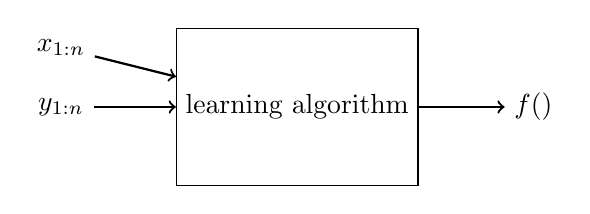
\begin{tikzpicture}
				
				\node(x) at (0, 0) [] {$x_{1:n}$};
				\node(y) at (0, -0.75) [] {$y_{1:n}$};
				
				
				\node(lr) at (3,-0.75) [draw, minimum width=2cm, minimum height=2cm]{learning algorithm};
				
				\draw[->,thick] (x) to (lr);
				\draw[->,thick] (y) to (lr);
				
				\node(f) at (6.0, -0.75) [] {$f()$};
				\draw[->,thick] (lr) to (f);
				
				\end{tikzpicture}
			\end{figure}

\end{frame}

\begin{frame}{Training as Optimization}
Loss function $L(y,\hat{y})$ quantifies the loss suffered when predicting $\hat{y}$ while the true label is $y$


Find the values of the parameters such that the overall loss $\mathcal{L}$ is minimized
\begin{equation*}
	\argmin_{\theta} \frac{1}{n}\sum_{i=1}^{n}L(\hat{y},y_i) 
\end{equation*}

\end{frame}


\begin{frame}{Logistic loss (Binary cross entropy)}

Assumes a set of two target classes labeled 0 and 1, with a correct label $y\in \{0, 1\}$
\begin{equation*}
L_{\text{logistic}} (\hat{y}, y) = -y \log(\hat{y}) -(1-y) \log(1-\hat{y})
\end{equation*}

Model output $\tilde{y}$ transformed using the \textbf{sigmoid function}
			\begin{equation*}
				\sigma(x) = \frac{1}{1+e^{-x}}
			\end{equation*}

Binary classification with conditional probability outputs:
$\hat{y} = \sigma(\tilde{y}) = \Pr(y=1|x)$

Inference rule: prediction$=0$ if $\hat{y}<0.5$ and prediction $=1$ if $\hat{y} \geq 0.5$

\end{frame}


\begin{frame}{Categorical cross-entropy loss}

True labels $y$ for each example is a vector = probability distribution over $C$ classes

Prediction vector $\hat{y}$ transformed through \textbf{softmax}

$$
\hat{y}[i] = \frac{\exp(z_{[i]})}{\sum_{j = 1}^{|C|} \exp(z_{[j]})}
$$

$$
L_{\text{cross-entropy}} (\hat{y}, y) = - \sum_{i = 1}^{|C|} y_{[i]} \log(\hat{y}_{[i]})
$$

\end{frame}


\iffalse
\begin{frame}{Regularization}
	\begin{itemize}
		
		\item<1-> to counter that we define a regularization term $R(\Theta)$ taking as input the parameters and returning a scalar that reflect their ``complexity,'' which we want to keep low
		
		\item<2-> training 
		\begin{equation*}
			\hat{\Theta} = \text{argmin}_{\Theta} \mathcal{L}(\Theta) =\text{argmin}_{\Theta} \frac{1}{n}\sum_{i=1}^{n}L(\hat{y},y_i) 
		\end{equation*}
		
		\item<3-> training with regularization
		\begin{equation*}
			\hat{\Theta} = \text{argmin}_{\Theta} \mathcal{L}(\Theta) =\text{argmin}_{\Theta} \left( \frac{1}{n}\sum_{i=1}^{n}L(\hat{y},y_i)  + \lambda R(\Theta) \right)
		\end{equation*}
	\end{itemize}
\end{frame}
\begin{frame}{Regularization}
	\begin{itemize}
		\item<1-> intuitively we would like to drive the learner toward natural solutions, in which it is OK to mis-classify a few examples if they don’t fit well with the rest
		\begin{equation*}
			\hat{\Theta} =\text{argmin}_{\Theta} \left( \frac{1}{n}\sum_{i=1}^{n}L(\hat{y},y_i)  + \lambda R(\Theta) \right)
		\end{equation*}
		\item<2-> regularization term considers the parameter values, and scores their complexity
		\item<3-> in practice the regularizers equate complexity with large weights and work to keep the parameter values low 
		
	\end{itemize}
\end{frame}
\begin{frame}{Common Regularization Functions}
	\begin{itemize}
		\item<1-> $L_2$ regularization (a.k.a. gaussian prior or weight decay): It keeps the sum of the squares of the parameter values low
		\begin{equation*}
			R_{L_2}(W) = ||W||_2^2 = \sum_{i,j}{(W_{[i,j]})^2}
		\end{equation*}
		\item<2-> the learner will prefer to decrease the value of one parameter with high weight by $1$ than to decrease the value of ten parameters that already have relatively low weights by $0.1$ each
	\end{itemize}
\end{frame}
\begin{frame}{Common Regularization Functions}
	\begin{itemize}
		\item<1-> $L_1$ regularization (a.k.a. sparse prior or lasso): It keeps  the sum of the absolute values of the parameters low
		\begin{equation*}
			R_{L_1}(W) = ||W||_1 = \sum_{i,j}{|W_{[i,j]}|}
		\end{equation*}
		\item<2-> the learner will prefer to decrease all the non-zero parameter values toward zero
	\end{itemize}
\end{frame}
\begin{frame}{Common Regularization Functions}
	\begin{itemize}
		\item<1-> Elastic-Net: combines both $L_1$ and $L_2$ regularization
		\begin{equation*}
			R_{\text{elastic-net}}(W) = \gamma_1 R_{L_1}(W) + \gamma_2 R_{L_2}(W)
		\end{equation*}
		\item<2-> dropout: will be discussed later
	\end{itemize}
\end{frame}
\fi


\section{Training as optimiziation}

\begin{frame}{Gradient-based Optimization}
\begin{figure}
	\centering
	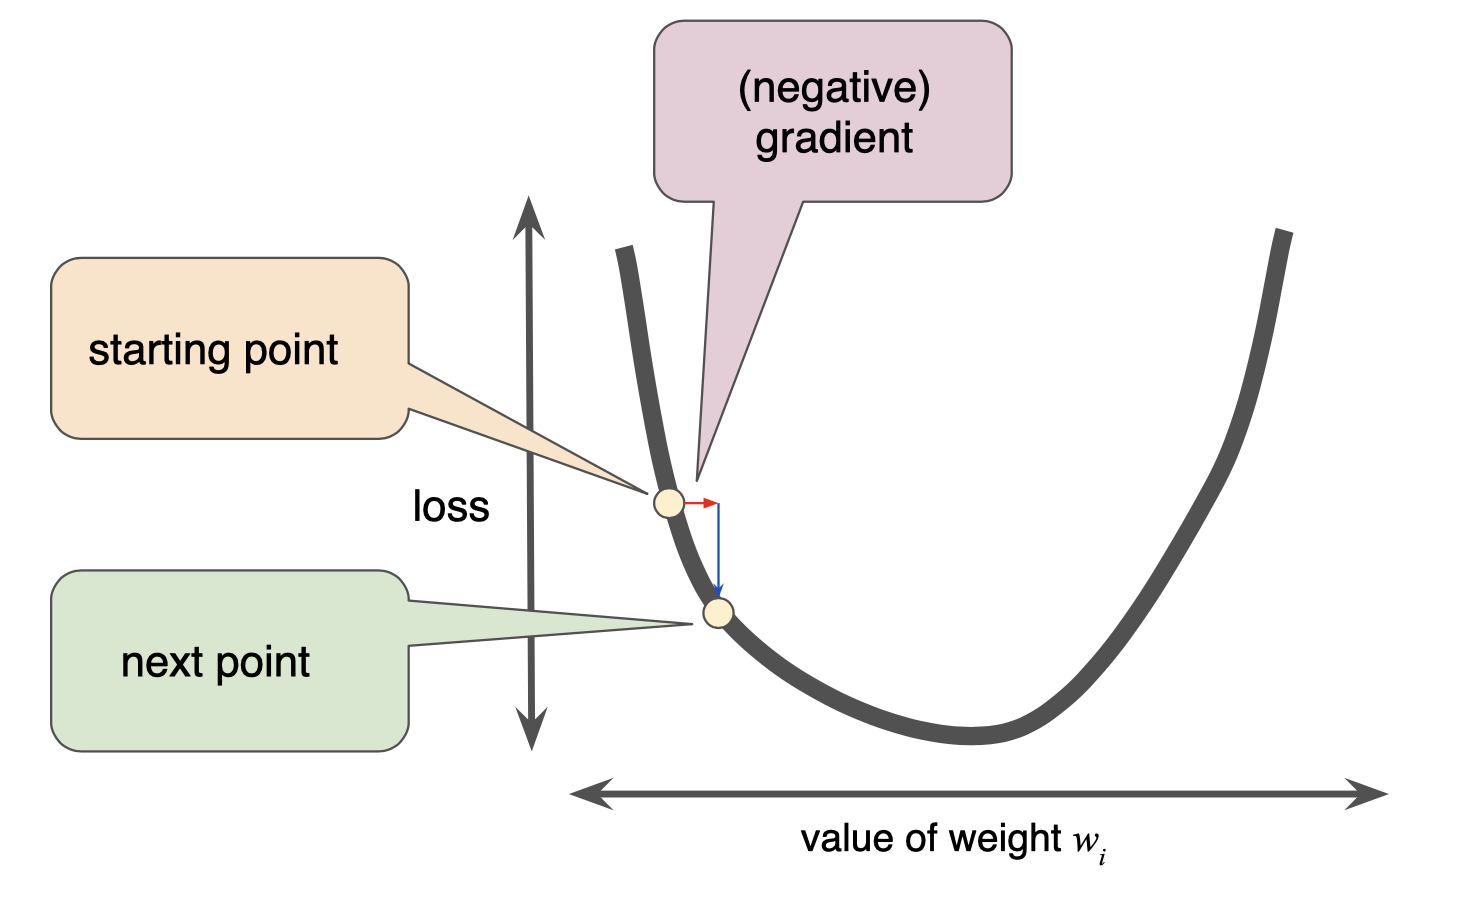
\includegraphics[width=0.8\linewidth]{img/sgd4.png}
\end{figure}
	
\end{frame}
\begin{frame}{Gradient-based Optimization}

Compute the loss over the training set

Compute the gradient of the loss with respect to the parameters

Update parameter values in the opposite directions of the gradient

\end{frame}

\begin{frame}{(Online) Stochastic Gradient Descent}

\hspace*{-2em}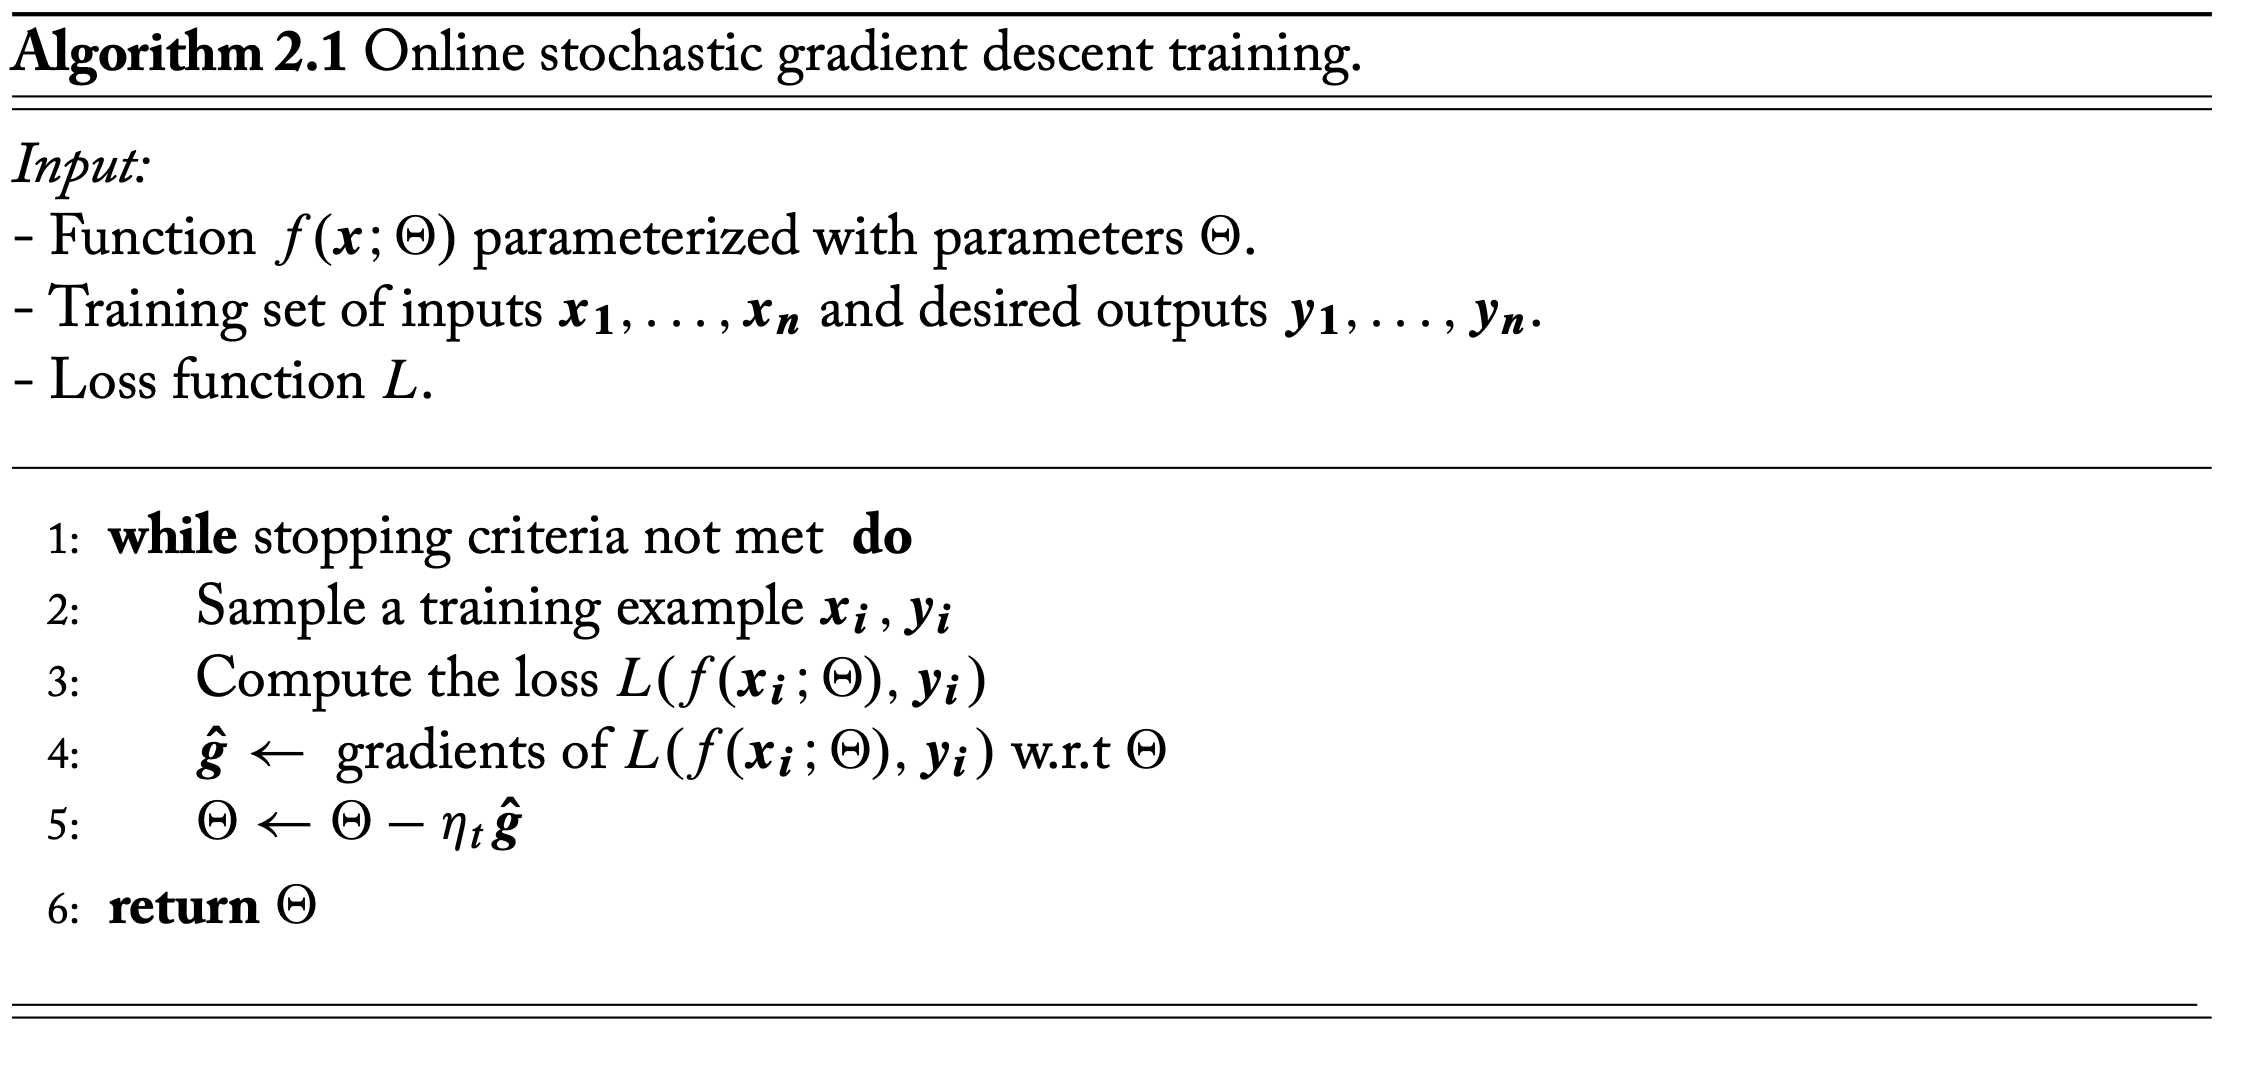
\includegraphics[width=1.15\linewidth]{img/sgd.png}
\vspace*{\fill}
\textit{\tiny{(Taken from: Neural Network Methods for Natural Language Processing, Yoav Goldberg)}}
\end{frame}

\begin{frame}{(Minibatch) Stochastic Gradient Descent}
	\centering
	\begin{figure}
		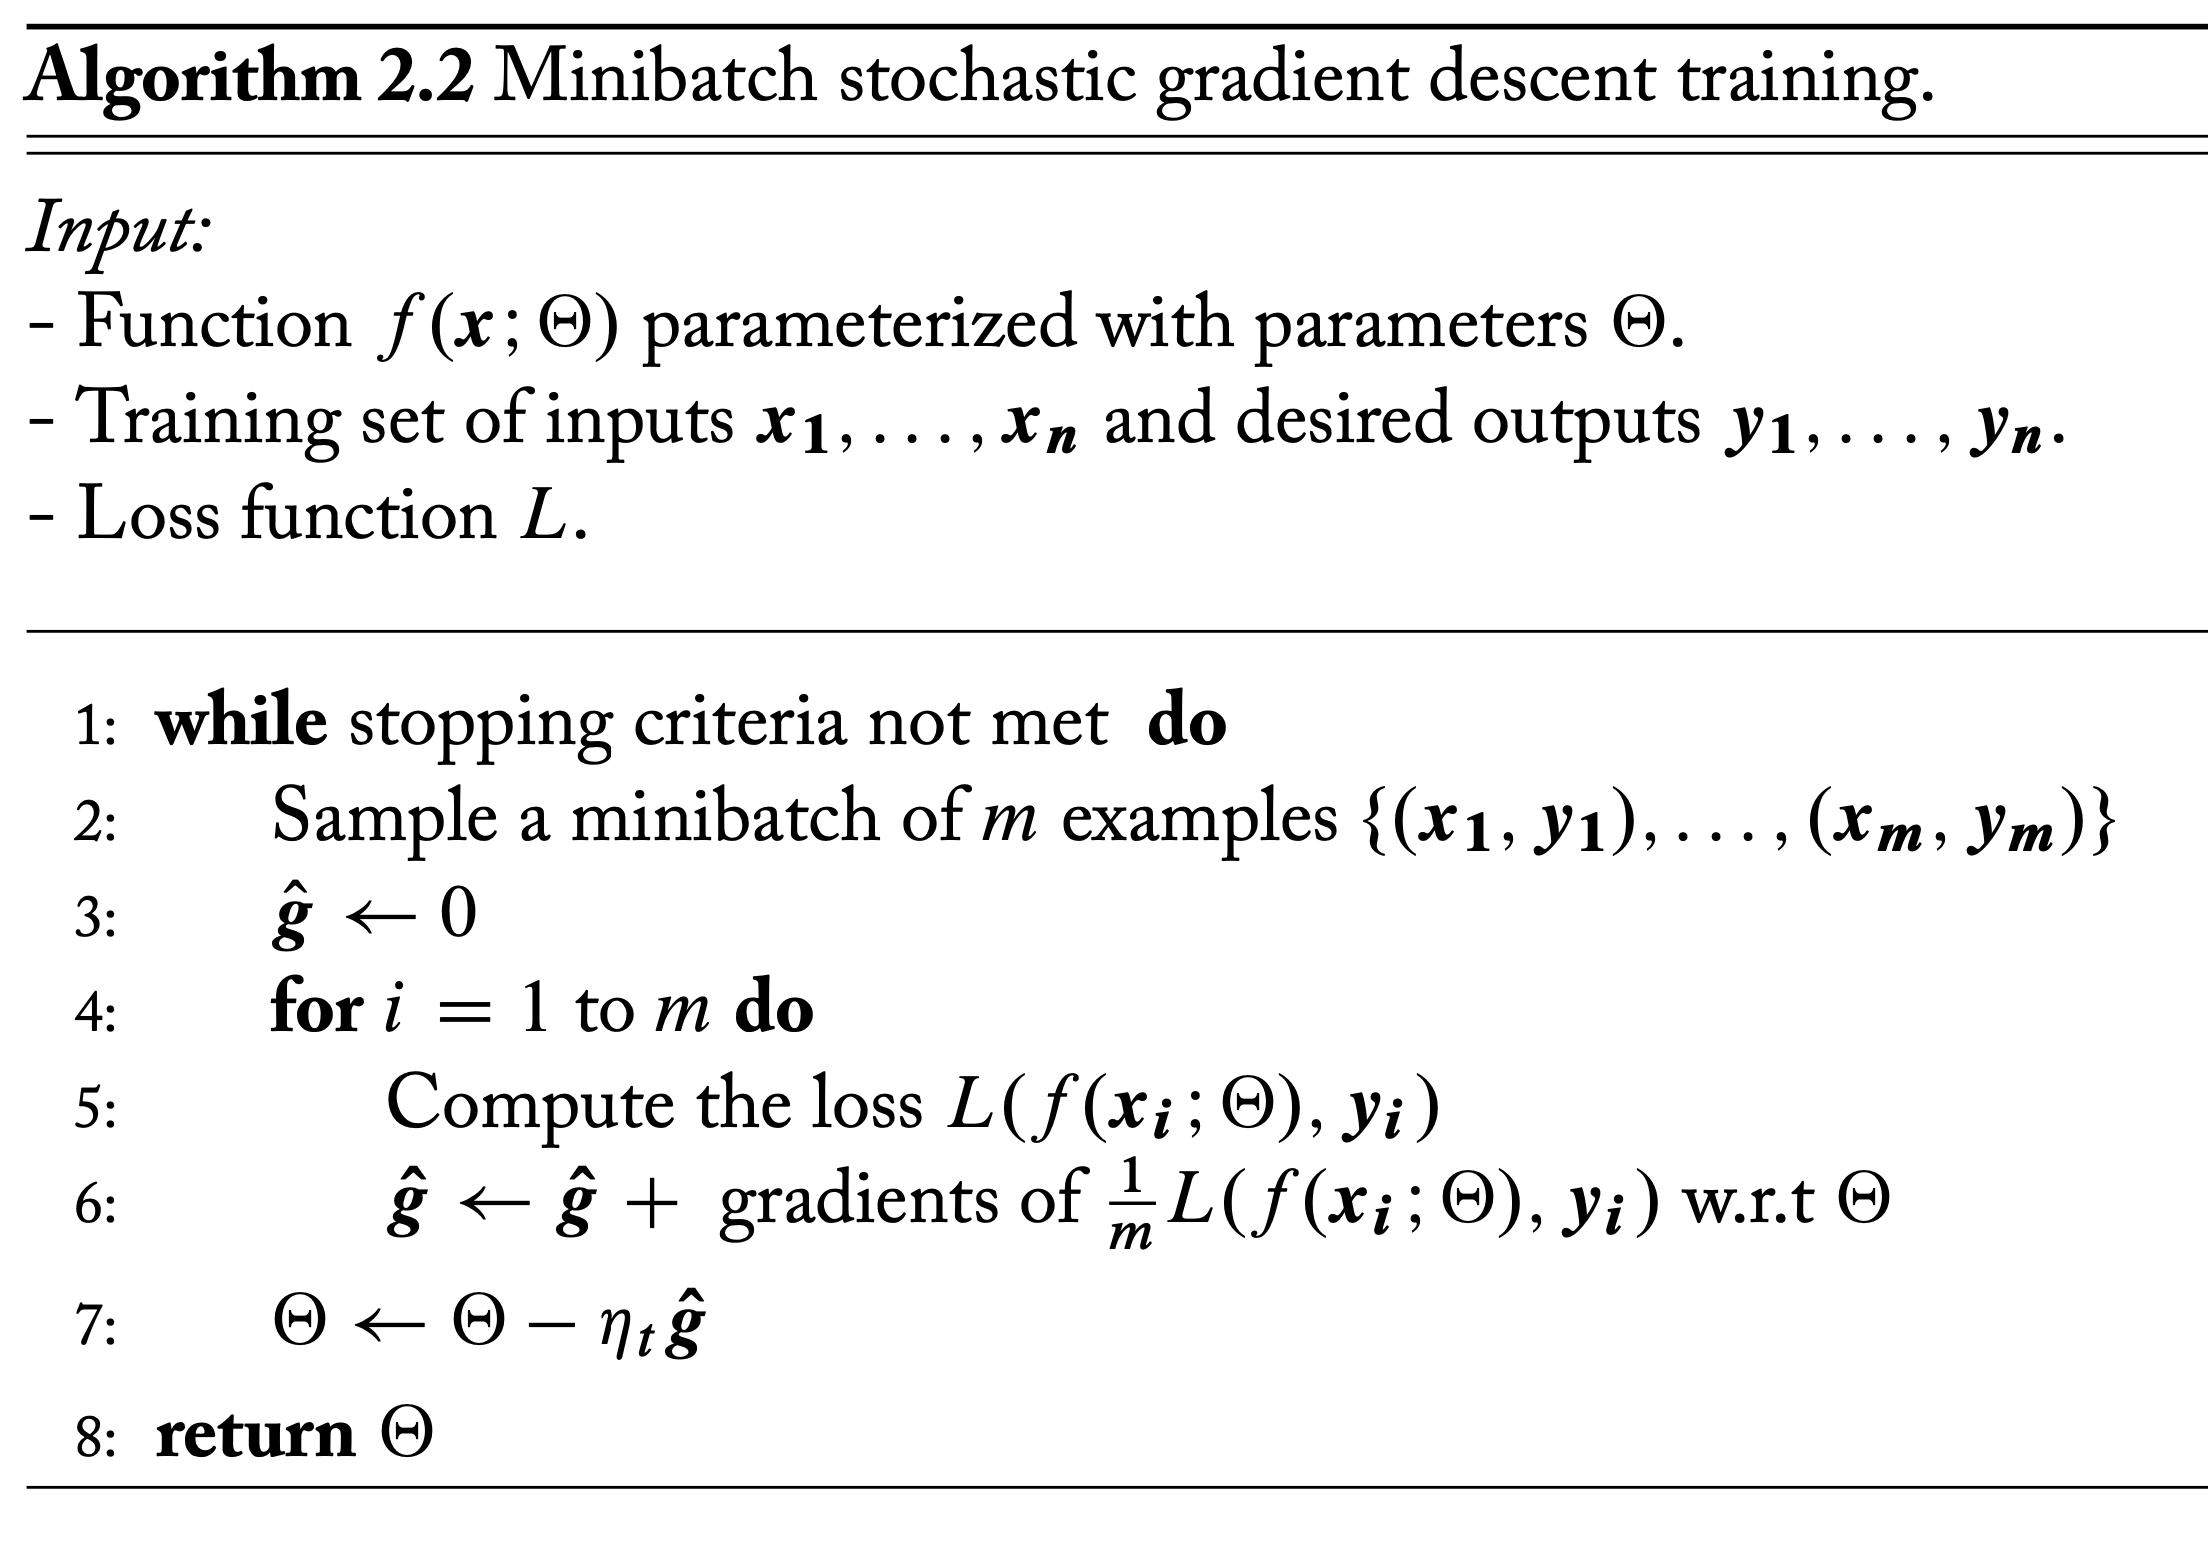
\includegraphics[width=\linewidth]{img/msgd.png}
	\end{figure}
	\vspace*{\fill}
	\textit{\tiny{(Taken from: Neural Network Methods for Natural Language Processing, Yoav Goldberg)}}
\end{frame}

\begin{frame}{Why Minibatch SGD?}

Less expensive than computing gradient on all training examples and then update

Converges empirically faster to a good solution than full-batch learning

\end{frame}

\begin{frame}{Small Learning Rate}
	\begin{figure}
		\centering
		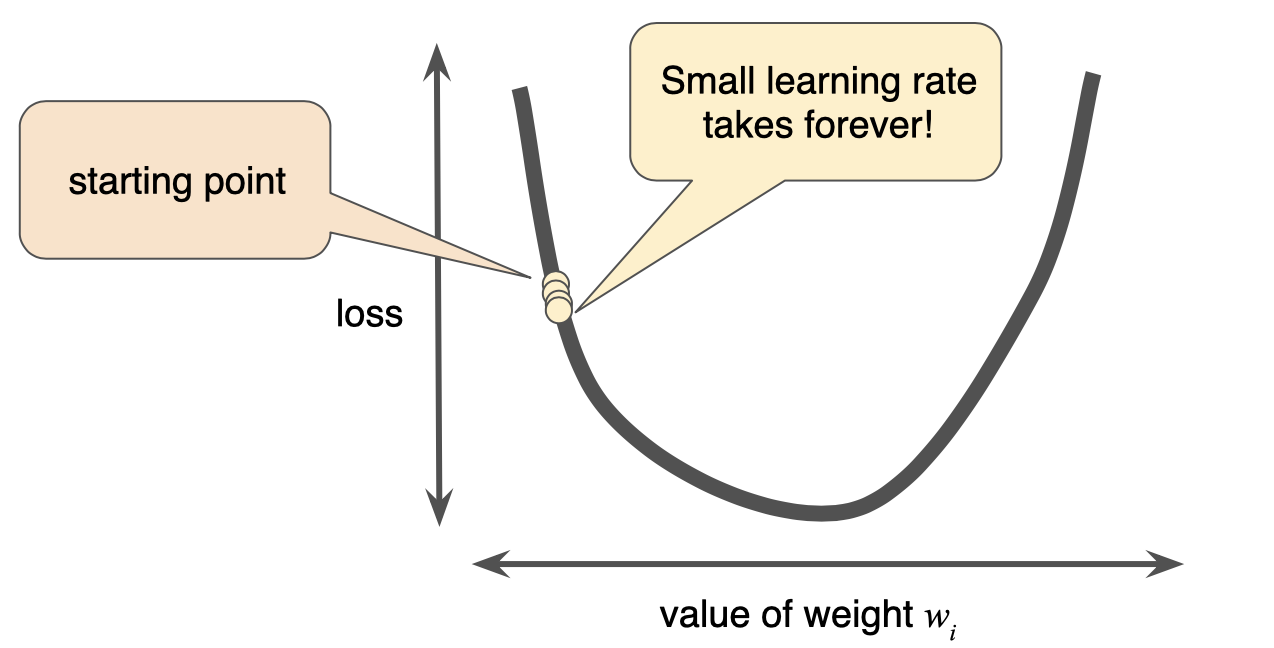
\includegraphics[width=0.8\linewidth]{img/small_lr.png}
	\end{figure}


\end{frame}
\begin{frame}{Large Learning Rate}
	\begin{figure}
		\centering
		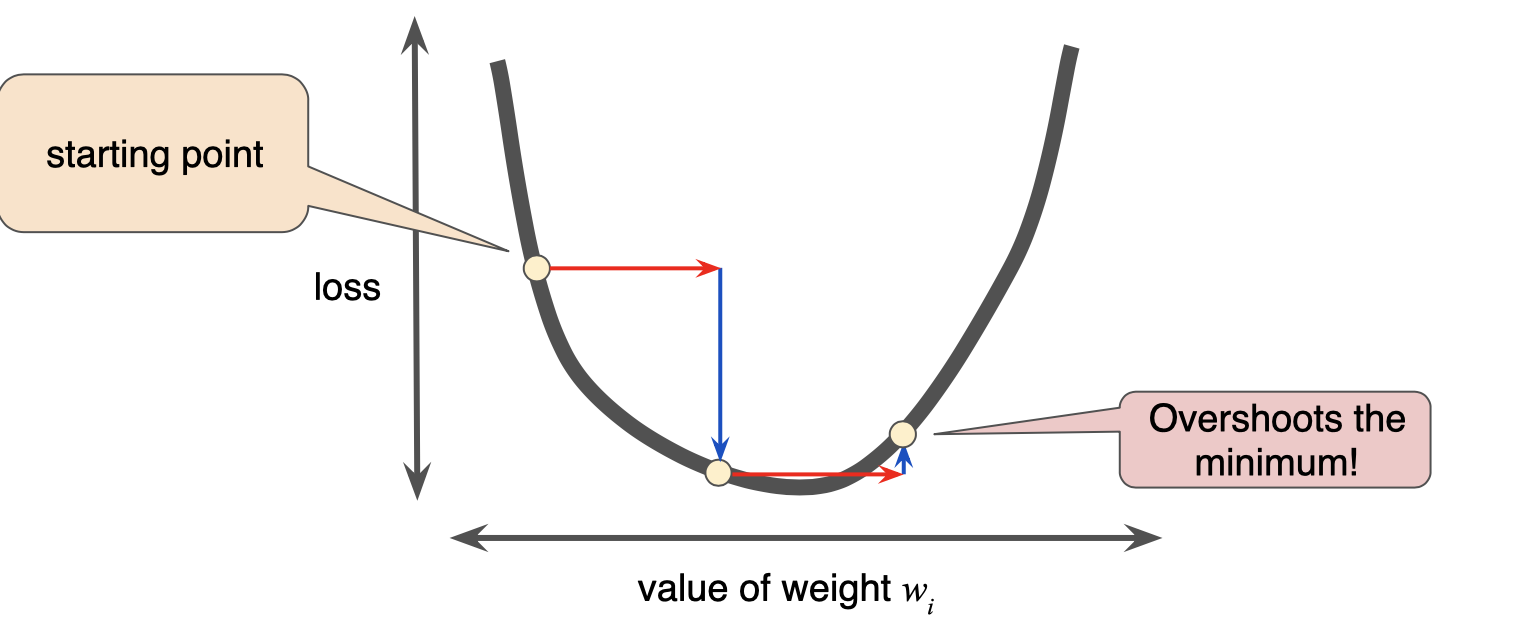
\includegraphics[width=\linewidth]{img/large_lr.png}
	\end{figure}

\end{frame}
\begin{frame}{Adaptive Learning Rate}
	\begin{figure}
		\centering
		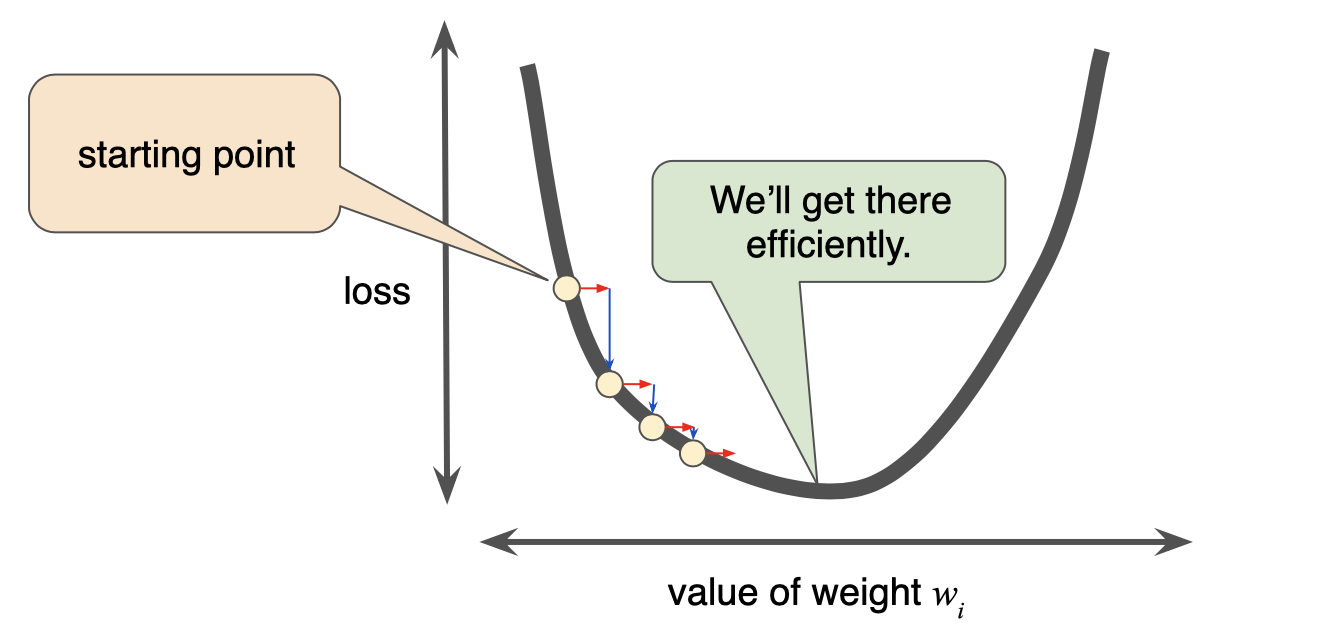
\includegraphics[width=0.8\linewidth]{img/adaptive_lr.png}
	\end{figure}

\begin{itemize}
	\item Adam \citep{Kingma.Ba.2015}
	\item AdaGrad [Duchi et al., 2011]
	\item AdaDelta [Zeiler, 2012]
	\item RMSProp [Tieleman and Hinton, 2012]
\end{itemize}

These methods train usually faster than SGD

\end{frame}

\section{Backpropagation}

\begin{frame}{Backpropagation}
	\begin{itemize}
		\item Recursive algorithm that computes the derivatives of a nested functions using the chain rule, while caching intermediary derivatives 
		\item Chain rule: Let $L = f(g(w))$
		\begin{equation*}
		\frac{\partial L}{\partial w} = \frac{\partial f}{\partial g}\times \frac{\partial g}{\partial w}   = \frac{\partial f}{\partial g}\frac{\partial g}{\partial w}
		\end{equation*}
	\end{itemize}
\end{frame}

\begin{frame}{Chain rule example}

Consider $y=e^{\sin(x^{2})}$

\bigskip

\begin{columns}
	\begin{column}{0.5\linewidth}
$y = f(u) = e^u$ \\
$u = g(v) = \sin v = \sin (x^2)$ \\
$v = h(x) = x^2$
	\end{column}
	\begin{column}{0.5\linewidth}
$\frac{dy}{du} = f'(u) = e^u = e^{\sin(x^{2})}$ \\
$\frac{du}{dv} = g'(v) = \cos v = \cos (x^2)$ \\
$\frac{dv}{dx} = h'(x) = 2x$
	\end{column}
\end{columns}

\bigskip


Derivative at the point $x = a$ is (in Leibniz notation)
$$
{\frac {dy}{dx}}=\left.{\frac {dy}{du}}\right|_{u=g(h(a))}\cdot \left.{\frac {du}{dv}}\right|_{v=h(a)}\cdot \left.{\frac {dv}{dx}}\right|_{x=a}
$$
	
\end{frame}

\begin{frame}{Backpropagation}

Consists of two steps

\begin{itemize}
	\item Forward pass $\rightarrow$ use current parameter values to compute the loss value
	\item Backward pass $\rightarrow$ use the gradient of the loss to update the parameter values
\end{itemize}

\end{frame}

\begin{frame}{Model: Multilayer Perceptron (MLP) }
	\centering
	\scalebox{0.8}{
		\begin{tikzpicture}
		\uncover<1->{
			\node[] (x) at (0,0) {$x$};
			\node[draw, minimum height=2, minimum width=3] (l1) at (0,1) {$ f \left( x W^{(1)} \right) $};
			\draw[->, thick] (x) -- (l1);
			
			\node[] (h1) at (0,4) {$h^{(1)}$}; 
			\draw[->, thick] (l1) -- (h1);
			
			\node[draw, minimum height=2, minimum width=3] (l2) at (0,5) {$ f \left( h^{(1)} W^{(2)} \right) $};
			\draw[->, thick] (h1) -- (l2);
			
			
%			\node[] (h2) at (0,8) {$h^{(2)}$}; 
%			\draw[->, thick] (l2) -- (h2);
%			
%			\node[draw, minimum height=2, minimum width=3] (l3) at (0,9) {$ f \left( h^{(2)} W^{(3)} \right) $};
%			\draw[->, thick] (h2) -- (l3);
			
			\node[] (y_hat) at (0,8) {$\hat{y}$}; 
			\draw[->, thick] (l2) -- (y_hat);
			
			\node[draw, white] (dummy-node) at (22,0) {};
		}
		\end{tikzpicture}
	}
\end{frame}

\iffalse
\begin{frame}{Backpropagation: Forward Pass}
	\centering
	\scalebox{0.5}{
		\begin{tikzpicture}
		\uncover<1->{
			\node[] (x) at (0,0) {$x$};
			\node[draw, minimum height=2, minimum width=3] (l1) at (0,1) {$ x W^{(1)} $};
			\draw[->, thick] (x) -- (l1);
			\node[] (z1) at (0,2) {$z^{(1)}$}; 
			\draw[->, thick] (l1) -- (z1);
		}
		\uncover<2->{
			\node[draw, minimum height=2, minimum width=3] (f1) at (0,3) {$ f\left( z^{(1)} \right)$};
			\draw[->, thick] (z1) -- (f1);
			\node[] (h1) at (0,4) {$h^{(1)}$}; 
			\draw[->, thick] (f1) -- (h1);
		}
		\uncover<3->{
			
			\node[draw, minimum height=2, minimum width=3] (l2) at (0,5) {$ h^{(1)} W^{(2)} $};
			\draw[->, thick] (h1) -- (l2);
			\node[] (z2) at (0,6) {$z^{(2)}$}; 
			\draw[->, thick] (l2) -- (z2);
			
			\node[draw, minimum height=2, minimum width=3] (f2) at (0,7) {$ f\left( z^{(2)} \right)$};
			\draw[->, thick] (z2) -- (f2);
			\node[] (yhat) at (0,8) {$\hat{y}$}; 
			\draw[->, thick] (f2) -- (yhat);
			
		}
%		\uncover<4->{
%			\node[draw, minimum height=2, minimum width=3] (l3) at (0,9) {$ h^{(2)} W^{(3)} $};
%			\draw[->, thick] (h2) -- (l3);
%			\node[] (z3) at (0,10) {$z^{(3)}$}; 
%			\draw[->, thick] (l3) -- (z3);
%			\node[draw, minimum height=2, minimum width=3] (f3) at (0,11) {$ f\left( z^{(3)} \right)$};
%			\draw[->, thick] (z3) -- (f3);
%			\node[] (y_hat) at (0,12) {$\hat{y}$}; 
%			\draw[->, thick] (f3) -- (y_hat);
%		}
		
		\uncover<5->
		{
			\node[draw] (loss) at (0,9) {$\mathcal{L}(y,\hat{y})$};
			\draw[->, thick, dashed] (yhat) -- (loss);
			\node[] (l) at (0,10) {$\ell$}; 
			\draw[->, thick] (loss) -- (l);
		}  
		
		\node[draw, white] (dummy-node) at (22,0) {};
		\end{tikzpicture}
	}
\end{frame}
\fi
% specific color for the next diagram
%\definecolor{myblue}{RGB}{1,70,153}

\begin{frame}
	\centering
	\scalebox{0.9}{
		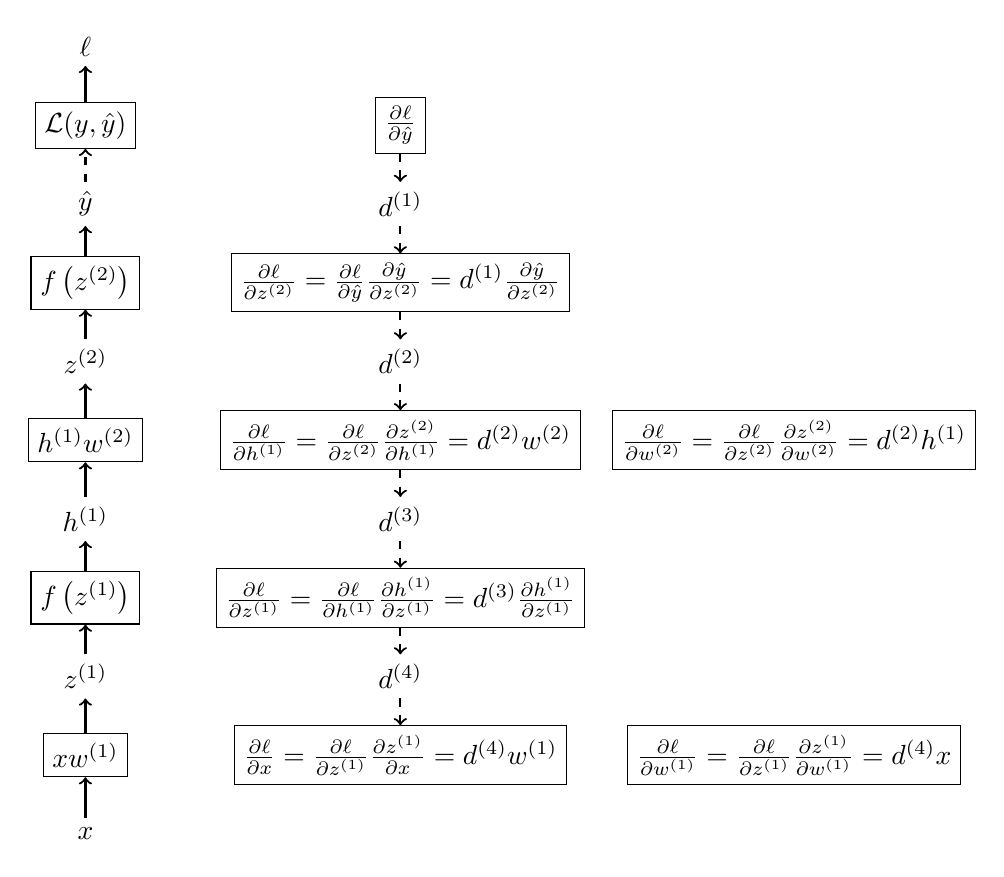
\begin{tikzpicture}
		
		\node[] (x) at (0,0) {$x$};
		\node[draw, minimum height=2, minimum width=3] (l1) at (0,1) {$ x w^{(1)} $};
		\draw[->, thick] (x) -- (l1);
		\node[] (z1) at (0,2) {$z^{(1)}$}; 
		\draw[->, thick] (l1) -- (z1);
		\node[draw, minimum height=2, minimum width=3] (f1) at (0,3) {$ f\left( z^{(1)} \right)$};
		\draw[->, thick] (z1) -- (f1);
		\node[] (h1) at (0,4) {$h^{(1)}$}; 
		\draw[->, thick] (f1) -- (h1);
		
%		\node[draw, minimum height=2, minimum width=3] (l2) at (0,5) {$ h^{(1)} w^{(2)} $};
%		\draw[->, thick] (h1) -- (l2);
%		\node[] (z2) at (0,6) {$z^{(2)}$}; 
%		\draw[->, thick] (l2) -- (z2);
		
		\node[draw, minimum height=2, minimum width=3] (l2) at (0,5) {$ h^{(1)} w^{(2)} $};
		\draw[->, thick] (h1) -- (l2);
		\node[] (z2) at (0,6) {$z^{(2)}$}; 
		\draw[->, thick] (l2) -- (z2);
		
		\node[draw, minimum height=2, minimum width=3] (f2) at (0,7) {$ f\left( z^{(2)} \right)$};
		\draw[->, thick] (z2) -- (f2);
		\node[] (yhat) at (0,8) {$\hat{y}$}; 
		\draw[->, thick] (f2) -- (yhat);
		
		\node[draw] (loss) at (0,9) {$\mathcal{L}(y,\hat{y})$};
		\draw[->, thick, dashed] (yhat) -- (loss);
		\node[] (l) at (0,10) {$\ell$}; 
		\draw[->, thick] (loss) -- (l);	
		
		
			\node[draw] (dl-dy_hat) at (4,9) {$\frac{\partial \ell }{\partial \hat{y}} $};
			\node[] (d1) at (4,8) {$d^{(1)}$};
			\draw[->, thick, dashed] (dl-dy_hat) -- (d1); 

			
			\node[draw] (dl-dz2) at (4,7) {$\frac{\partial \ell}{ \partial z^{(2)}} = \frac{\partial \ell}{ \partial \hat{y}} \frac{\partial \hat{y}}{ \partial z^{(2)} } = d^{(1)} \frac{\partial \hat{y}}{ \partial z^{(2)} }
				$};
			\draw[->, thick, dashed] (d1) -- (dl-dz2);

			\node[] (d4) at (4,6) {$d^{(2)}$};
			\draw[->, thick, dashed] (dl-dz2) -- (d4); 
			
			\node[draw] (dl-dh1) at (4,5) {$\frac{\partial \ell}{ \partial h^{(1)}} = \frac{\partial \ell}{ \partial z^{(2)}} \frac{\partial z^{(2)}}{ \partial h^{(1)} } = d^{(2)} w^{(2)}
				$};
			\draw[->, thick, dashed] (d4) -- (dl-dh1);

			\node[draw] (dl-dw2) at (9,5) {$\frac{\partial \ell}{ \partial w^{(2)}} = \frac{\partial \ell}{ \partial z^{(2)}} \frac{\partial z^{(2)}}{ \partial w^{(2)} } = d^{(2)} h^{(1)}
				$};
			
			\node[] (d5) at (4,4) {$d^{(3)}$};
			\draw[->, thick, dashed] (dl-dh1) -- (d5); 
			
			\node[draw] (dl-dz1) at (4,3) {$\frac{\partial \ell}{ \partial z^{(1)}} = \frac{\partial \ell}{ \partial h^{(1)}} \frac{\partial h^{(1)}}{ \partial z^{(1)} } = d^{(3)} \frac{\partial h^{(1)}}{ \partial z^{(1)} }
				$};
			\draw[->, thick, dashed] (d5) -- (dl-dz1);

			\node[] (d6) at (4,2) {$d^{(4)}$};
			\draw[->, thick, dashed] (dl-dz1) -- (d6); 
			
			\node[draw] (dl-dx) at (4,1) {$\frac{\partial \ell}{ \partial x} = \frac{\partial \ell}{ \partial z^{(1)}} \frac{\partial z^{(1)}}{ \partial x } = d^{(4)} w^{(1)}
				$};
			\draw[->, thick, dashed] (d6) -- (dl-dx);
			
			\node[draw] (dl-dw1) at (9,1) {$\frac{\partial \ell}{ \partial w^{(1)}} = \frac{\partial \ell}{ \partial z^{(1)}} \frac{\partial z^{(1)}}{ \partial w^{(1)} } = d^{(4)} x
				$};

		\end{tikzpicture}
	}
\end{frame}

\begin{frame}{Backprop + SGD}

Output of backprop is gradient wrt.\ parameters of the neural network

Once we have the gradient we can use SGD rule to update the parameter values

\end{frame}



\section{Language models}


\begin{frame}{Language Models (LMs)}

Language modeling = assigning probability to a sentence in a language

Example: $\Pr(\text{`The cat sat on the mat .'})$

Ideal performance at language modeling: predict the next token in a sequence with a number of guesses that is the identical to or lower than the number of guesses required by a human

Crucial component in real-world NLP applications: conversational AI, machine-translation, text summarization, etc.

\end{frame}
\begin{frame}{Language Models (LMs)}

Assume a sequence of words $w_{1:n} = w_1 w_2 ... w_{n-1} w_n$

$$
\begin{aligned}
\Pr(w_1, w_2, \ldots, w_{n-1}, w_n) = &\Pr(w_1) \cdot \\
& \Pr(w_2|w_1) \cdot \\
& \Pr(w_3|w_1, w_2) \cdot \\
& \Pr(w_4|w_1, w_2, w_3) \cdot \\
& \ldots \cdot \Pr(w_n|w_{1:n-1})
\end{aligned}
$$

Each word is predicted conditioned on the preceding words

Probability of the last token conditioned on $n-1$ preceding words


	
\end{frame}
\begin{frame}{Markov assumption}

$k$th order Markov-assumption: next word in a sequence depends only on the last $k$ words
		\begin{equation*}
		\Pr(w_{i}|w_{1:i-1}) \approx \Pr(w_i | w_{(i-1)-k:i-1})
		\end{equation*}

Probability of a sequence of tokens $w_{1:n}$
		\begin{equation*}
		\Pr(w_{1:n}) \approx \prod_{i=1}^{n} \Pr(w_i | w_{i-k:i-1})
		\end{equation*}

Computationally-friendly version (What is the problem with the above formula?)
\pause
\begin{equation*}
\log_2 \Pr(w_{1:n}) \approx \sum_{i=1}^{n} \log_2 \left( \Pr(w_i | w_{i-k:i-1} )\right)
\end{equation*}


\end{frame}
\begin{frame}{Evaluating language models}

\textbf{Perplexity}: How well a LM predicts likelihood of unseen sentence

		\begin{equation*}
		\text{Perp}_{w_{1:n}} (\text{LM}) = 2^{-\frac{1}{n} \sum_{i=1}^{n} \log_2 \text{LM}({w_i|w_{1:i-1}})}
		\end{equation*}

Low perplexity values $\to$ better language model (assigns high probabilities to the unseen sentences)
		
We can compare several language models with one another

Perplexities of two language models are only comparable with respect to the same evaluation dataset

\end{frame}
\begin{frame}{Estimating Probabilities}

Count-based: The estimates can be derived from corpus counts


Let $\#(w_{i:j})$ be the count of the sequence of words $w_{i:j}$ in a corpus

The maximum likelihood estimate (MLE) of $\Pr(w_{i}|w_{i-1-k:i-1})$
		\begin{equation*}
		\Pr(w_{i}|w_{i-1-k:i-1}) = \frac{\#(w_{i-1-k:i})}{\#(w_{i-1-k:i-1})}
		\end{equation*}

Example: $w_1w_2w_3 =$ the cat sat
		\begin{equation*}
		\Pr(w_{3}|w_{1:2}) = \frac{\#(\text{the cat sat})}{\#(\text{the cat})}
		\end{equation*}

\end{frame}
\begin{frame}{Estimating Probabilities}

What if $\#(w_{i:j}) =0 $?  

\pause

$\to$ infinite perplexity 

One way of avoiding zero-probability N-grams is to use smoothing techniques

Additive smoothing: assume $|V|$ is  the vocabulary size and $0<\alpha \leq 1$
\begin{equation*}
\Pr(w_{i}|w_{i-1-k:i-1}) = \frac{\#(w_{i-1-k:i}) + \alpha}{\#(w_{i-1-k:i-1}) + \alpha|V|}
\end{equation*}
		

\end{frame}
\begin{frame}{Pro and Cons of Discussed LMs}
Easy to train, scale to large corpora, and work well in practice

Scaling to larger N-grams is a problem for MLE-based language models. 

Large number of words in the vocabulary means that statistics for larger N-grams will be sparse

MLE-based language models suffer from lack of generalization across contexts

Having observed ``black car'' and ``blue car'' does not influence our estimates of the sequence ``red car'' if we haven’t seen it before

\end{frame}
\begin{frame}{Neural Language Models}

Use neural networks to estimate probabilities of a LM

We can overcome the shortcomings of the MLE-based LMs because neural networks 
		\begin{itemize}
			\item enable conditioning on increasingly large context sizes with only a linear increase in the number of parameters
			\item support generalization across different contexts
		\end{itemize}

We focus on the neural LM that was introduced by \citep{Bengio.et.al.2003.JMLR}

\end{frame}
\begin{frame}{Neural Language Models}

Let $w_{1:k}$ be the given context

We want to estimate $\Pr(w_{k+1}|w_{1:k})$

Design an MLP neural net, which takes $w_{1:k}$ as input and returns $\Pr(w_{k+1})$ over all words in vocabulary $V$ as output
$$
\begin{aligned}		
x  &= [v(w_1), v(w_2), ..., v(w_k)] \\
h^{(1)} &= g(xW^{(1)}+b^{(1)}) \\
\Pr(w_{k+1}) &= \text{softmax}(h^{(1)}W^{(2)}+b^{(2)})
\end{aligned}
$$

Training examples: word k-grams from the training set, where the identities of the first $k-1$ words are used as features. Last word: target label for the classification

Loss function: cross-entropy loss

\end{frame}

\begin{frame}{(Neural) LMs for language generation}
	
Assume that we are given $w_{1:k}$ as context

Predict the next word $w_{k+1}$ from vocabulary $V$

Feed $w_{1:k}$ to our trained MLP-based LM 

Our LM returns $\Pr(w_{k+1})$ of each word in $V$ 

Pick the word with the maximum probability to generate the next word

Add the the predicted word to the context and repeat the above procedure
	
\end{frame}


\begin{frame}[allowframebreaks]{References}
\printbibliography
%  \bibliography{demo}
%  \bibliographystyle{abbrv}
\end{frame}

\begin{frame}{License and credits}
	
	\begin{columns}
		\begin{column}{0.7\textwidth}
			Licensed under Creative Commons Attribution-ShareAlike 4.0 International (CC BY-SA 4.0)
		\end{column}
		\begin{column}{0.2\textwidth}
			
\includegraphics[width=0.9\linewidth]{img/cc-by-sa-icon.pdf}
		\end{column}
	\end{columns}
	
	\bigskip
	
	Credits
	
	\begin{scriptsize}
		
		Ivan Habernal, Mohsen Mesgar, Steffen Eger
		
		Content from ACL Anthology papers licensed under CC-BY \url{https://www.aclweb.org/anthology}
		
		Pictures courtesy of 	\url{https://developers.google.com/machine-learning/crash-course/reducing-loss/gradient-descent}
		
	\end{scriptsize}
	
\end{frame}



\end{document}

